%! Author = paulsen
%! Date = 12.09.23

\begin{frame}{Software}
    \section{Software}\label{sec:software}
\end{frame}


\begin{frame}{Pakete}
    \subsection{Pakete}\label{subsec:pakete}

    Was sind (Software-)Pakete?
    \pause

    \vspace{0.5cm}
    \begin{quote}
        Eine Paketverwaltung ermöglicht die komfortable Verwaltung von Software, die in Form von Programmpaketen vorliegt
    \end{quote}
    \pause

    \begin{itemize}
        \item Pakete sind in einem Zentralen Repository hinterlegt\pause
        \item Ermöglicht strukturiertes Updaten\pause
        \item Kein Linux-Einheitliches Paketformat
    \end{itemize}
\end{frame}

\begin{frame}{Pakete}
    \subsection{Varianten}\label{subsec:varianten}

    \begin{enumerate}
        \item<1-> Distributions-Spezifische Paketformate
        \item<2-> Unabhängige Containerformate
        \item<3-> Sonstiges: Appimage, Nativ, Compiliert mit Sourcecode
    \end{enumerate}

    \vspace{0.5cm}
    \begin{exampleblock}<1->{Fun Fact}
        Android hat "APK" als einheitliches Paketformat
    \end{exampleblock}

\end{frame}

\begin{frame}{Spezifische Paketformate}
    \subsubsection{}\label{subsubsec:spezifische-formate}

    \minipage{0.49\textwidth}
        Distributionsspezifische Paketmanager die auf System-Level laufen:
        \begin{itemize}
            \item<2-> APT
            \item<3-> PACMAN
            \item<4-> DNF
            \item<5-> \ldots
        \end{itemize}
    \endminipage\hfill
    \minipage{0.49\textwidth}
        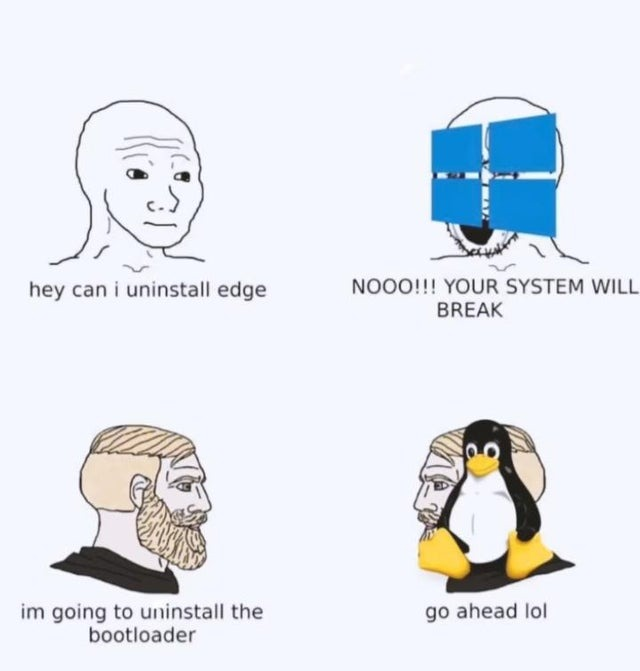
\includegraphics[width=\linewidth]{Meme_Uninstall-Bootloader}
    \endminipage\hfill
\end{frame}

\begin{frame}{Containerformate}
    \subsubsection{}\label{subsubsec:containerformate}

    Laufen System-Unabhängig und meistens auf Benutzer-Level
    \pause

    \begin{itemize}
        \item Flatpak\pause
        \item Snap\pause
        \item Docker
    \end{itemize}

\end{frame}

\begin{frame}{Sonstige Paketformate}
    \subsubsection{}\label{subsubsec:sonstige-paketformate}

    \begin{itemize}
        \item Appimage: Einzelne Datei beinhaltet die Anwendung und alles was es benötigt\pause
        \item Nativ: Anwendungs-Version ist nur für spezifische Geräteart (ARM-Prozessor, IOS, x86)\pause
        \item Quellcode: Beim Benutzer wird eine (seinem System) zugeschnittene Anwendung erstellt.
    \end{itemize}

\end{frame}

\begin{frame}{Software Installation}
    \subsection{Installation}\label{subsec:installation}

    \begin{itemize}
        \item Installation Grafisch oder über Konsole möglich\pause
        \item "Discover" kann Programme verschiedener Paketarten installieren
    \end{itemize}

\end{frame}

\begin{frame}{Discover}
    \subsubsection{Discover}\label{subsubsec:discover}

    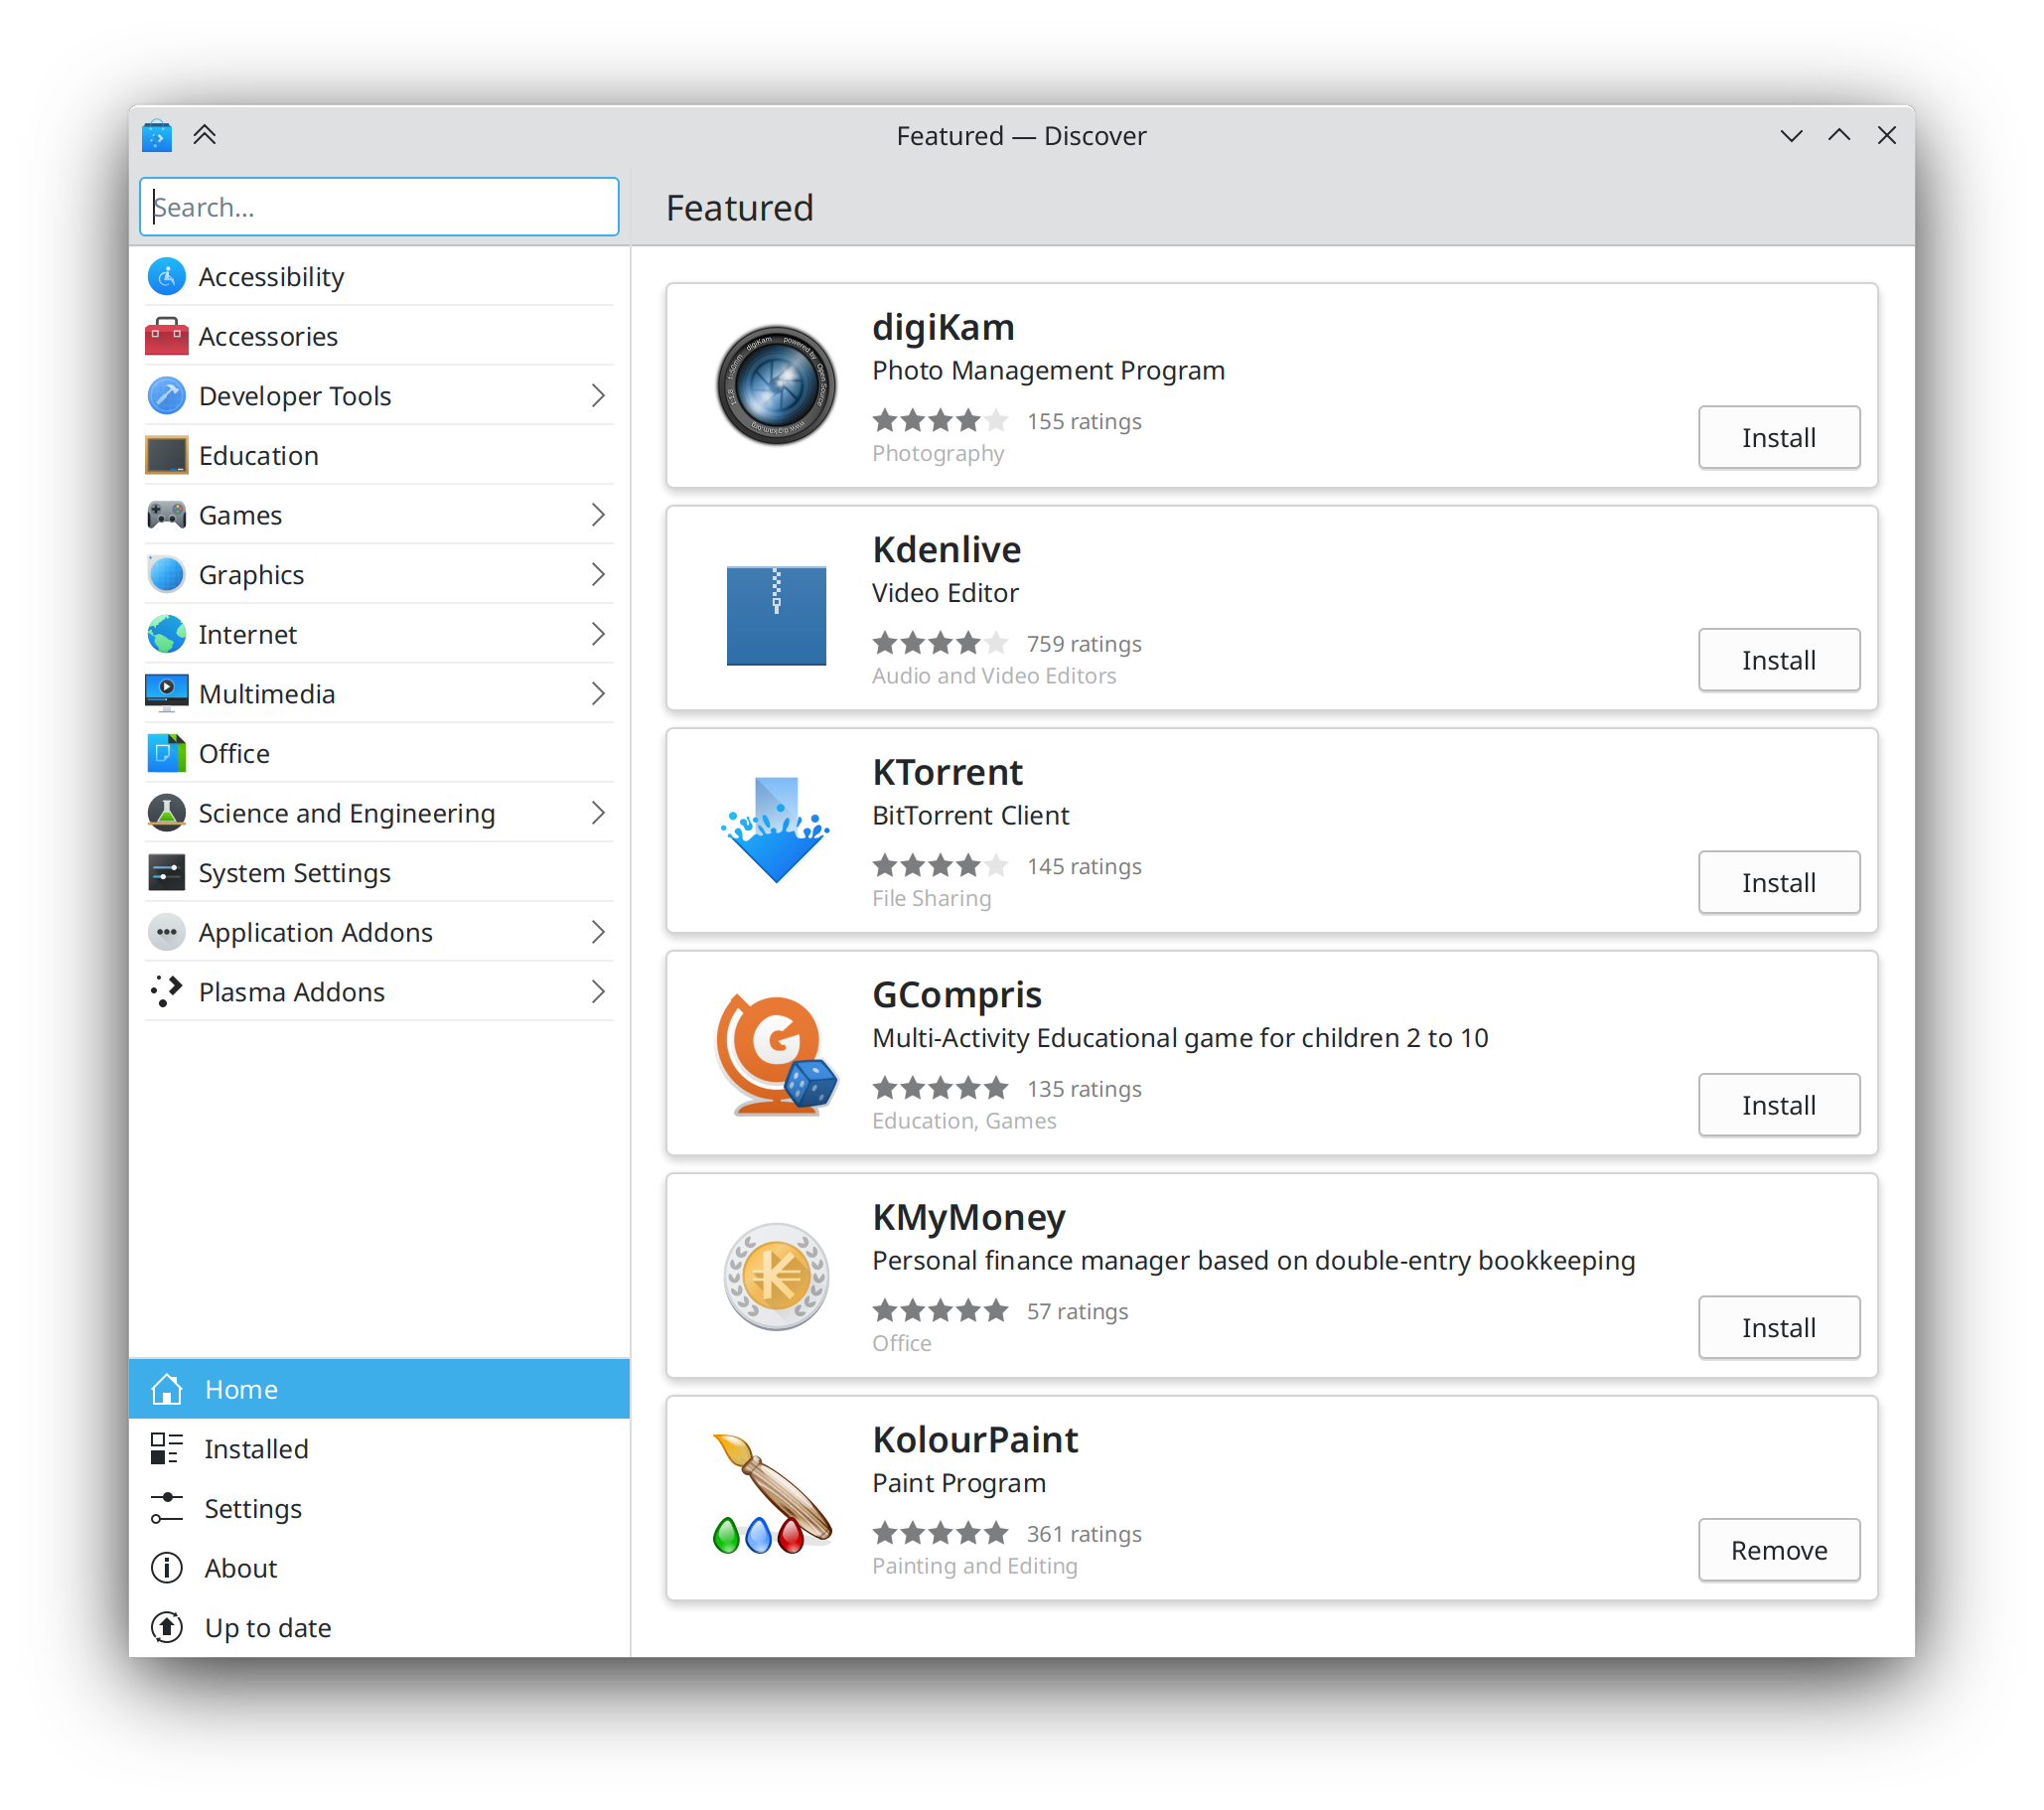
\includegraphics[width=10cm]{plasma-discover}
\end{frame}

\begin{frame}{Discover}
    \vspace{0.5cm}
    \begin{alertblock}{Aufgabe}
        Aktualisiere dein System.
    \end{alertblock}
    \pause

    \vspace{0.5cm}
    \begin{alertblock}{Aufgabe}
        Installiere folgende Programme:
        \begin{itemize}
            \item OnlyOffice
            \item Xournal++
        \end{itemize}
    \end{alertblock}

\end{frame}

\begin{frame}{Office}

    \begin{itemize}
        \item OnlyOffice: All-In-One Microsoft-Office Ersatz\pause
        \item Xournal++: Notizen\pause
        \item Okular: PDF-Reader und Formulare\pause
        \item PDFPC: Presenter
    \end{itemize}

\end{frame}

\begin{frame}{Office}
    \vspace{0.5cm}
    \begin{alertblock}{Aufgabe}
        \begin{enumerate}
            \item Erstelle ein Office-Dokument mithilfe von OnlyOffice.\pause
            \item Exportiere dieses Dokument als PDF.\pause
            \item Mache dich mit Xournal++ vertraut und unterschreibe das Dokument.\pause
            \item Exportiere das unterschriebene Dokument wieder als PDF.\pause
            \item Überprüfe mithilfe von Okular, ob das Dokument passt.
        \end{enumerate}
    \end{alertblock}
\end{frame}